\begin{frame}
	\frametitle{Herramientas y Tecnologías utilizadas}
	\block{ Android Studio}
		\begin{itemize}
			\item Entorno de desarrollo integrado.
			\item Gradle.
			\item Sistema de depuración sencillo e intuitivo.
		\end{itemize}
	\endblock{}
\end{frame}

%------------------------------------------------------------------
\begin{frame}
	\frametitle{Herramientas y Tecnologías utilizadas}
	\block{\it Realidad Aumentada (RA)}
		\begin{itemize}
			\item {\it ¿Qué es la RA?}.
			\item {\it ¿Cómo funciona esta tecnología?}.
			\item {\it ¿Qué tipos de Realidad Aumentada existen?}.
			\item {\it ¿Diferencias entre la Realidad Aumentada y la Realidad Virtual (RV)?}.
			\item {\it ¿Qué es la Realidad Mixta?}.
			\item {\it ¿Qué futuro le espera a la RA?}.
			\item {\it Integración de la RA en Android Studio}.
		\end{itemize}
	\endblock{}
\end{frame}

%------------------------------------------------------------------

\begin{frame}
	\frametitle{Herramientas y Tecnologías utilizadas}
		\block{\it ¿Qué es la realidad aumentada?}
		\begin{itemize}
			\item Permite expandir la información del mundo físico.
			\item Se encuentra en su mejor momento.
			\item Aplicaciones para todos los ámbitos. 
		\end{itemize}
		\endblock{}

		\begin{center}
			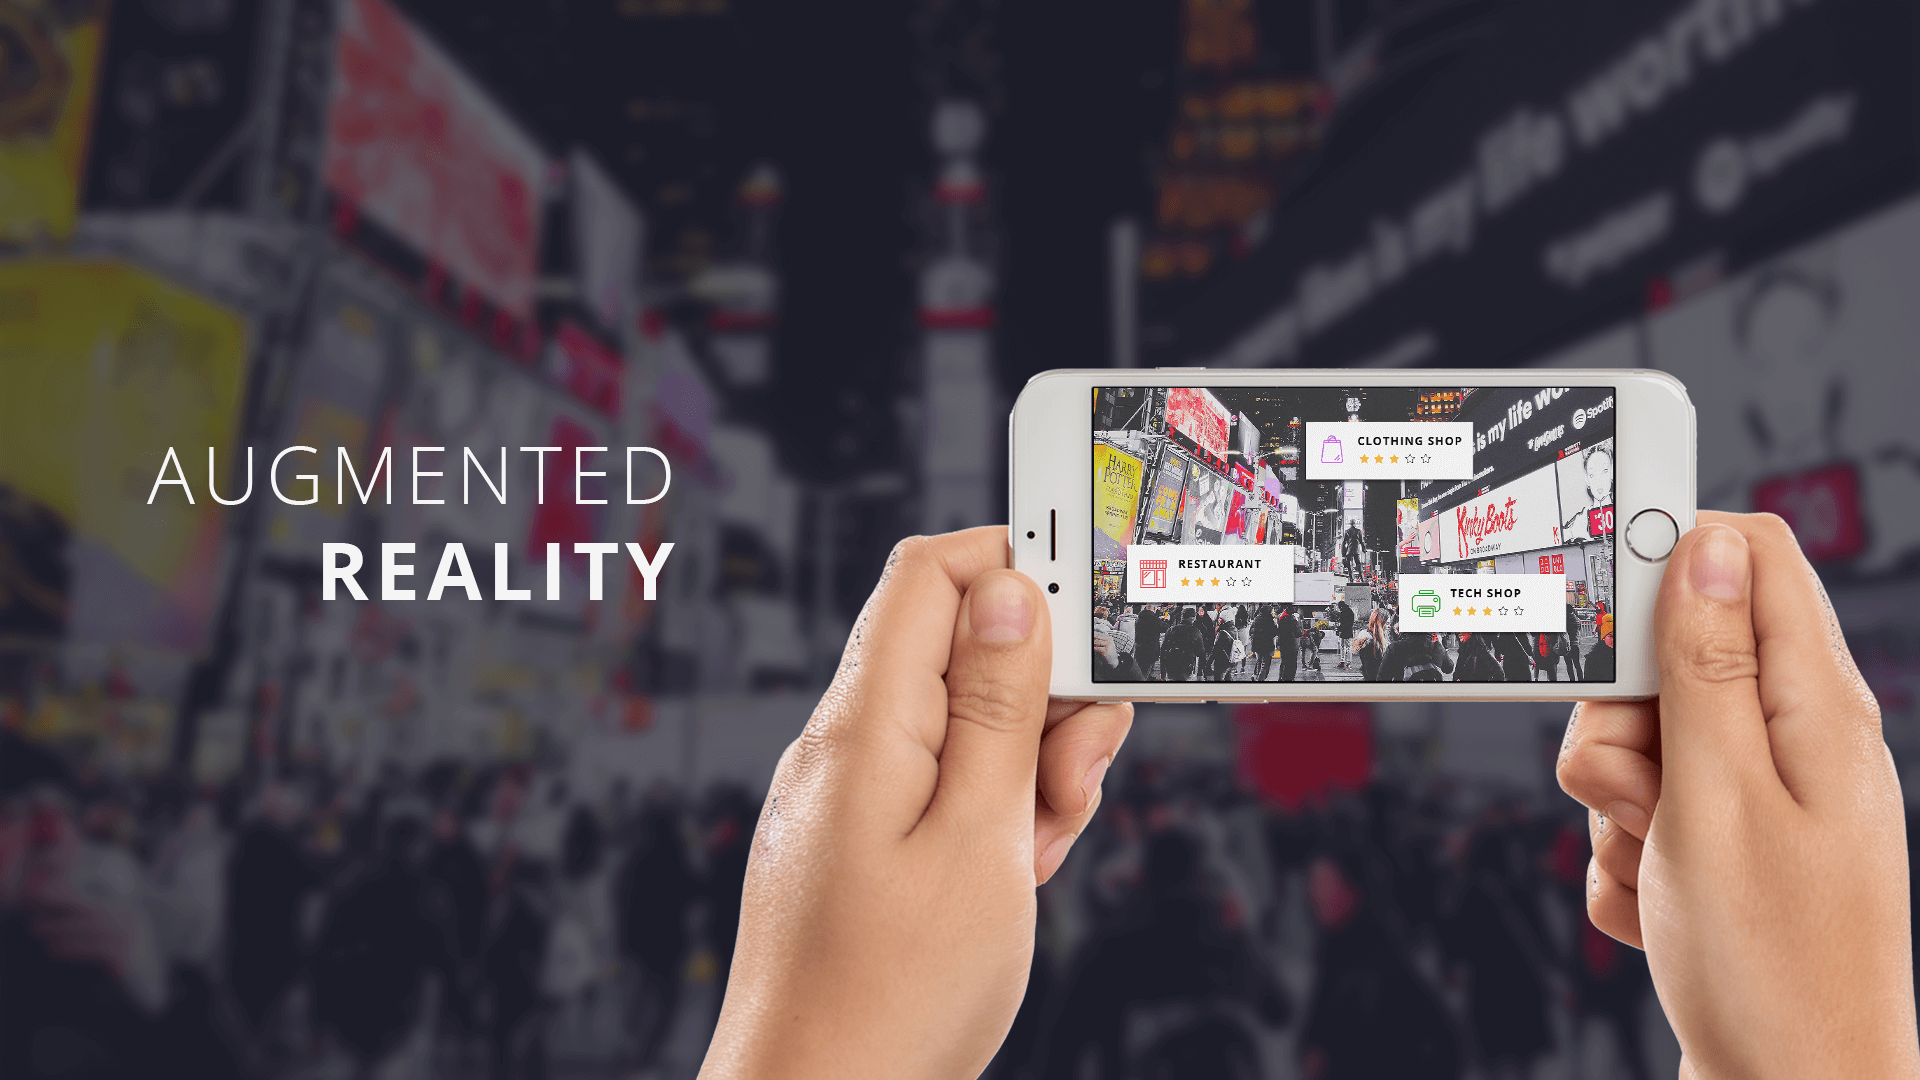
\includegraphics[width=0.7\linewidth]{Images/ar3}
		\end{center}
	
\end{frame}

%------------------------------------------------------------------
\begin{frame}
	\frametitle{Herramientas y Tecnologías utilizadas}
		\block{\it ¿Cómo funciona esta tecnología?}
			Componentes necesarios para la tecnología de RA:
			\begin{itemize}
				\item {Dispositivo de visualización.}
				\item {Sistema de computación.}
				\item {Sensores: GPS, WIFI, Bluetooth, acelerómetro, giroscopio, cámara, etc.}
				\item {Software de RA.}
			\end{itemize}
		\endblock{}

		\begin{center}
			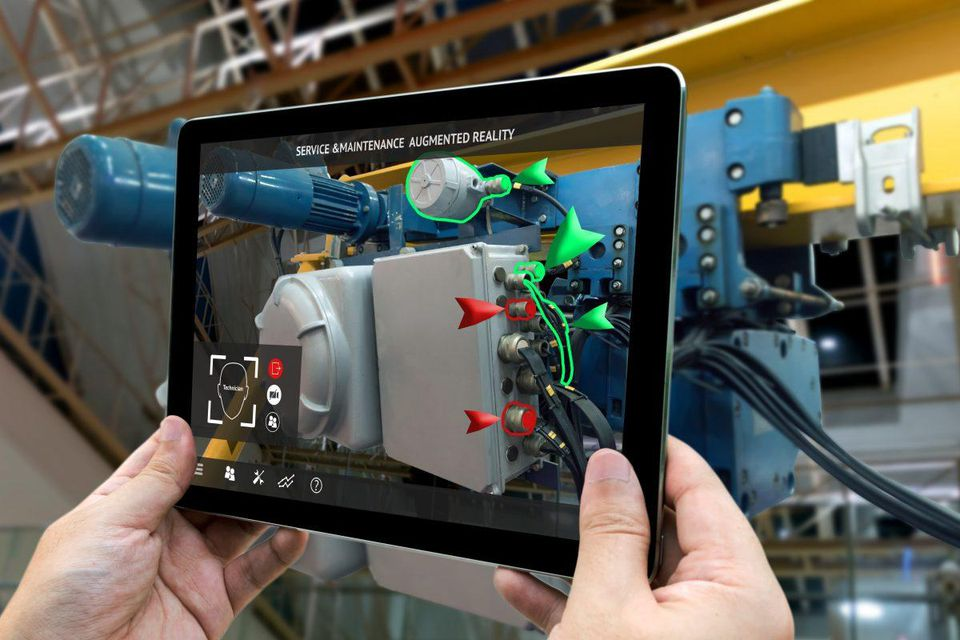
\includegraphics[width=0.43\linewidth]{Images/ar1}
		\end{center}
\end{frame}
		


\begin{frame}
	\frametitle{Herramientas y Tecnologías utilizadas}
	\begin{columns}
			\begin{column}{0.45\textwidth}
				\block{\it ¿Qué tipos de RA existen?}
					Existen distintos tipos de RA:
					\begin{itemize}
						\item {Marker-based AR.}
						\item {Markerless AR.}
						\item {Pojection-based AR.}
						\item {Superimposition-based AR.}
					\end{itemize}
				\endblock{}
			\end{column}
			\begin{column}{0.55\textwidth}
				\vfill 
					\begin{center}
						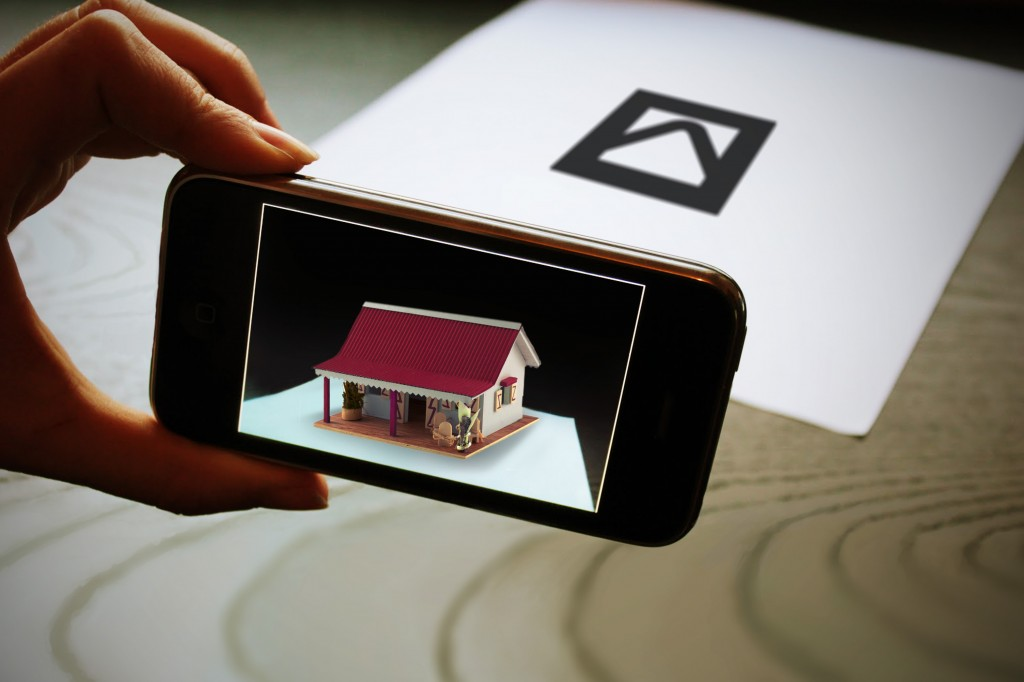
\includegraphics[width=0.95\linewidth]{Images/marker-ar}
					\end{center}
			\end{column}
	\end{columns}
\end{frame}

%------------------------------------------------------------------

\begin{frame}
	\frametitle{Herramientas y Tecnologías utilizadas}
		\block{\it ¿Diferencias entre la Realidad Aumentada y la Realidad Virtual (RV)?}
			\begin{itemize}
				\item {En la actualidad se encuentra más avanzada que la RA.}
				\item {Muestra al usuario un entorno de escenas y objetos de aperiencia real.}
				\item {Dispone de distintos mecanismos de interacción.}
				\item {Aleja al usuario del entorno real.}
			\end{itemize}
		\endblock{}
			\begin{center}
				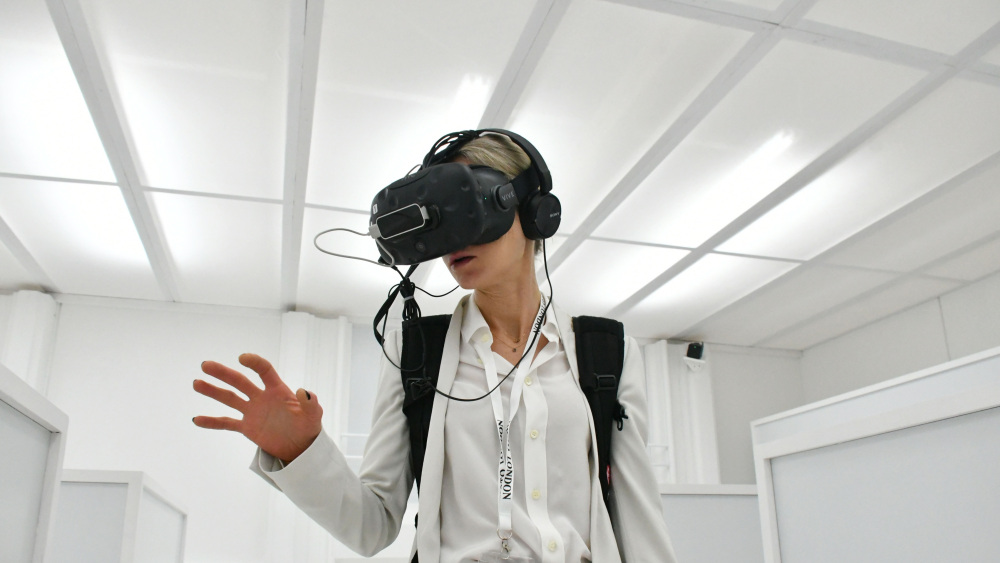
\includegraphics[width=0.50\linewidth]{Images/vr1}
			\end{center}
\end{frame}

%--------------------------------------------------------------------


\begin{frame}
	\frametitle{Herramientas y Tecnologías utilizadas}
		\block{\it ¿Qué es la Realidad Mixta?}
			\begin{itemize}
				\item {Es la union de la RA con la RV}.
				\item {Consiste en llevar el mundo real al mundo virtual.}
				\item {Requiere de mayor capacidad de procesamiento que la RA.}
			\end{itemize}
		\endblock{}
		\vfill 
			\begin{center}
				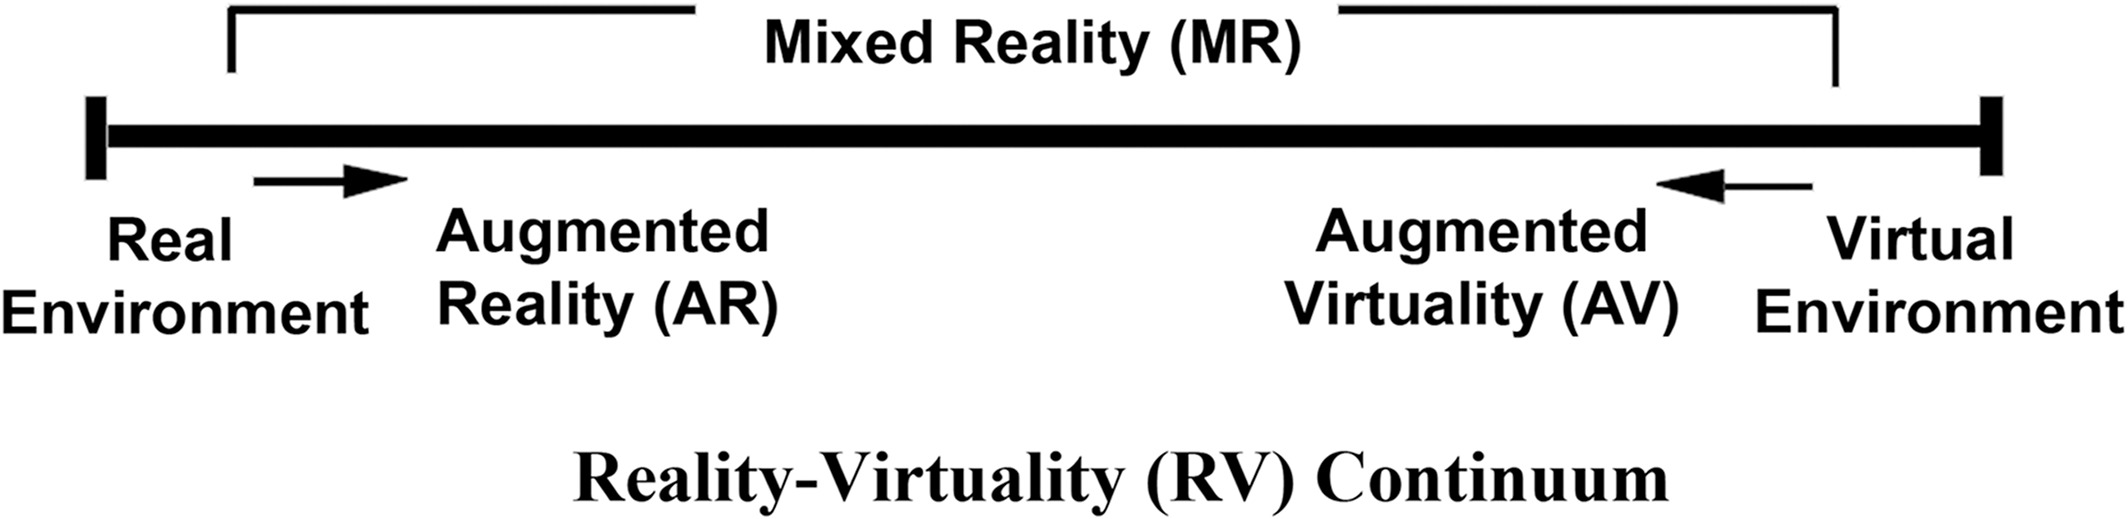
\includegraphics[width=0.8\linewidth]{Images/realidamixta}
			\end{center}
\end{frame}


\begin{frame}
	\frametitle{Herramientas y Tecnologías utilizadas}
	\block{\it ¿Qué futuro le espera a la Realidad Aumentada?}
		Los usos de la RA se acercan a todos los sectores:
		\begin{itemize}
			\item {Educación}.
			\item {Videojuegos.}
			\item {Industria.}
			\item {Turismo.}
			\item {Medicina.}
		\end{itemize}

	\endblock{}
\end{frame}



\begin{frame}
	\frametitle{Herramientas y Tecnologías utilizadas}
	\block{\it  Integración de la Realidad Aumentada en Android Studio}
		\begin{columns}
			\begin{column}{0.3\textwidth}
				\begin{center}					
					Vuforia 
				\end{center}
				\vspace{3mm}
				\vfill 
					\begin{center}
						
\includegraphics[width=0.8\linewidth]{Images/vuforia}
					\end{center}
			\end{column}
			\begin{column}{0.3\textwidth}
				\begin{center}
				Kudan AR SDK
				\end{center}
				\vspace{3mm}
				\vfill 
					\begin{center}
						
\includegraphics[width=0.8\linewidth]{Images/kudan}
					\end{center}
			\end{column}
			\begin{column}{0.3\textwidth}
				\begin{center}
					MaxST SDK
				\end{center}
				\vspace{3mm}
				\vfill 
					\begin{center}
						
\includegraphics[width=0.5\linewidth]{Images/maxst}
					\end{center}
			\end{column}
		\end{columns}
	\endblock{}
\end{frame}

\begin{frame}
	\frametitle{Herramientas y Tecnologías utilizadas}
		\block{\it Node.js}
			\begin{itemize}
				\item {¿Qué es?}.
				\item {¿Cómo funciona?}.
				\item {¿Por qué se ha decidido utilizar esta tecnología?}.
			\end{itemize}
		\endblock{}
		\vfill 
			\begin{center}
				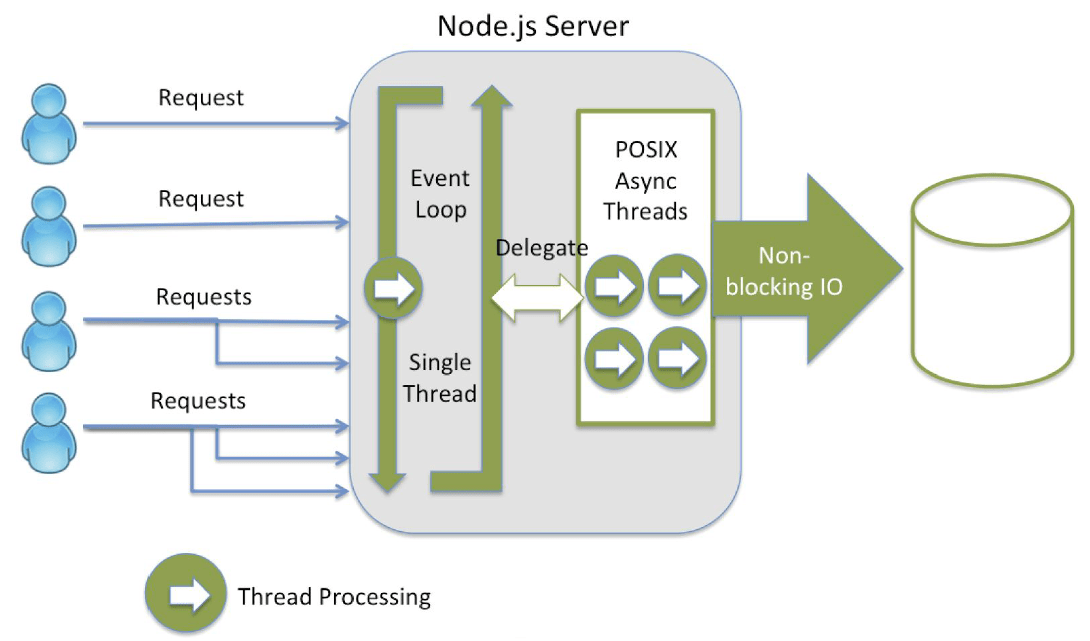
\includegraphics[width=0.72\linewidth]{Images/nodejsEx}
			\end{center}
\end{frame}

\begin{frame}
	\frametitle{Herramientas y Tecnologías utilizadas}
		\block{\it MongoDB}
			\begin{itemize}
				\item {Base de datos NoSQL}.
				\item {De esquema libre}.
				\item {¿Porqué se ha decidido utilizar MongoDB?}.
			\end{itemize}
		\endblock{}
		\vfill 
		\begin{center}
			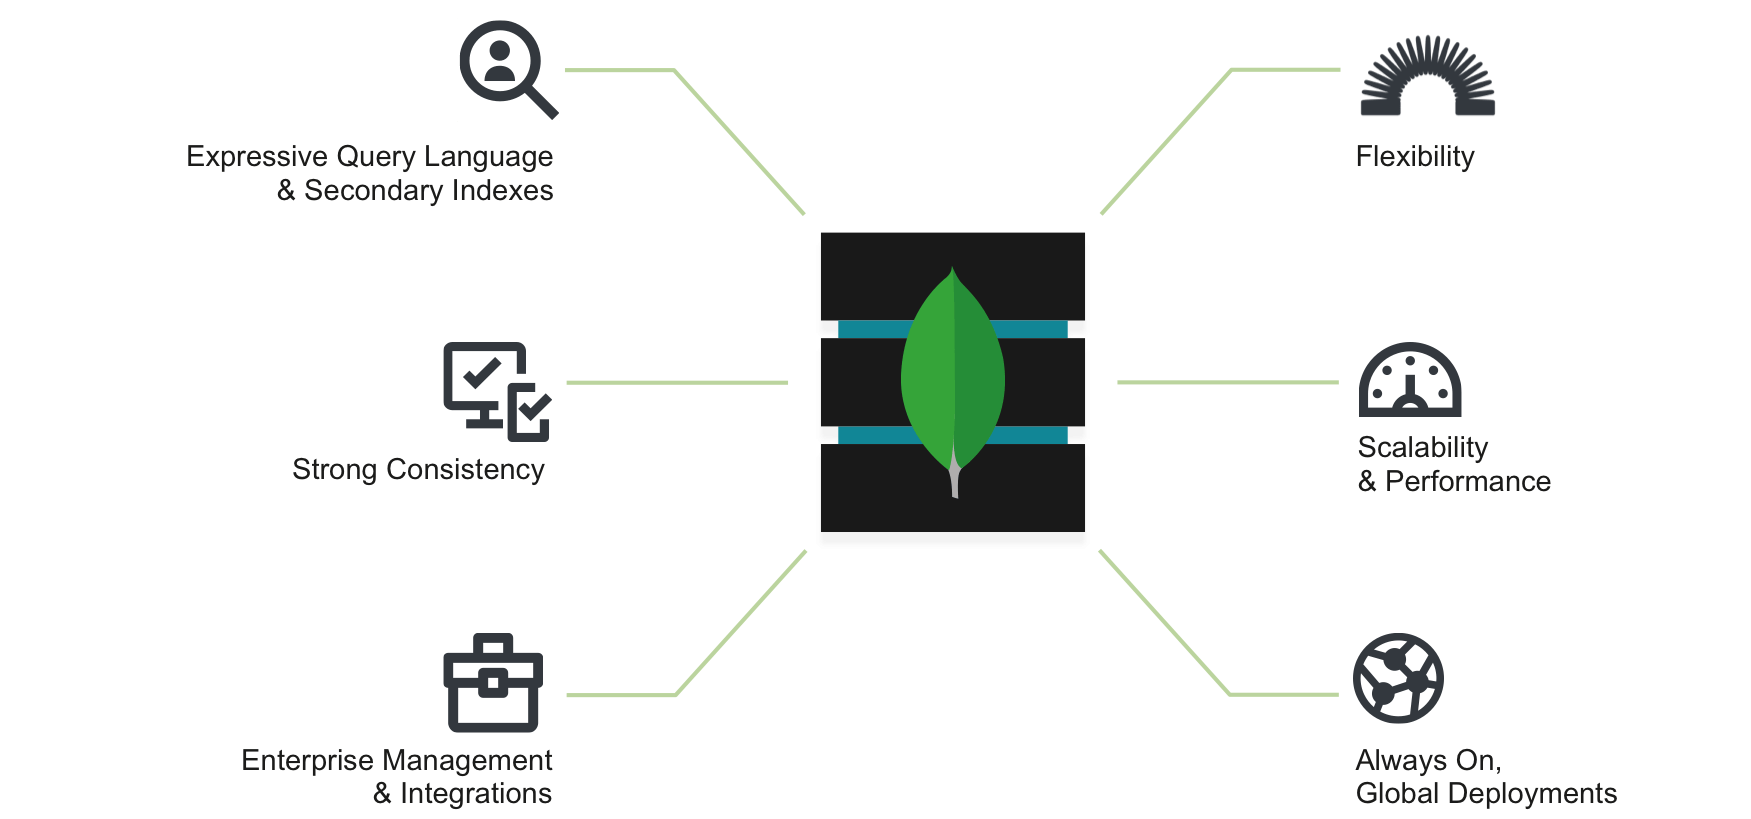
\includegraphics[width=0.88\linewidth]{Images/mongodb-architecture}
		\end{center}
\end{frame}

\begin{frame}
	\frametitle{Herramientas y Tecnologías utilizadas}
	\begin{columns}
			\begin{column}{0.6\textwidth}
				\block{\it Heroku}
					\begin{itemize}
						\item {Plataforma como servicio de computación (PaaS) en la nube}.
						\item {Soporta distintos lenguajes de programación}.
						\item {Ejecuta las aplicaciones en ``dynos''.}
						\item {Servidor de \ULLAR{}}.
					\end{itemize}
				\endblock{}
			\end{column}
			\begin{column}{0.4\textwidth}
				\vfill 
					\begin{center}
						
\includegraphics[width=0.9\linewidth]{Images/heroku}
					\end{center}
			\end{column}
	\end{columns}
\end{frame}

\begin{frame}
	\frametitle{Herramientas y Tecnologías utilizadas}
	\begin{columns}
			\begin{column}{0.6\textwidth}
				\block{\it mLab}
					\begin{itemize}
						\item {Servicio de base de datos como servicio en la nube}
						\item {Ofrece bases de datos MongoDB}.
						\item {Ejecuta sus máquinas en proveedores de servicios en la nube como AWS, Azure y Google Cloud.}
						\item {Base de datos de \ULLAR{}.}
					\end{itemize}
				\endblock{}
			\end{column}
			\begin{column}{0.4\textwidth}
				\vfill 
					\begin{center}
						
\includegraphics[width=0.8\linewidth]{Images/mlab}
					\end{center}
			\end{column}
	\end{columns}
\end{frame}

\begin{frame}
	\frametitle{Herramientas y Tecnologías utilizadas}
		\block{\it Google Maps}
			\begin{itemize}
				\item {API de Google Maps.}
				\item {Permite integrar los mapas de Google Maps en una aplicación Android.}
				\item {Permite:}
				\begin{itemize}
					\item {Creación de marcadores, polígonos y superposiciones.}
					\item {Cambiar la vista del mapa.}
					\item {La posibilidad de elegir el tipo de mapa}
				\end{itemize}
			\end{itemize}
		\endblock{}
\end{frame}

%--------------------------------------------------------------------
